 \PassOptionsToPackage{svgnames}{xcolor}
\documentclass[sigconf,nonacm,natbib=false,screen]{acmart}

\usepackage[utf8]{inputenc}
\usepackage[T1]{fontenc}
\usepackage[american]{babel}

\usepackage{csquotes}

\usepackage{subcaption}
\usepackage{newfloat}
\usepackage{xspace}

% Set up TiKZ and libraries
\usepackage{tikz}
\usetikzlibrary{fit}
\usetikzlibrary{positioning}

\PassOptionsToPackage{
  sortcites,
  maxcitenames=2,
  date=year,
  % From ACM sample file
  abbreviate=true,
  backend=biber,
  backref=false,
  dateabbrev=true,
  doi=true,
  isbn=true,
  language=american,
  maxbibnames=9,
  style=ACM-Reference-Format,
  url=true,
  urldate=comp,
}{biblatex}
\usepackage{biblatex}
%\bibliography{bibliography}

% Setup hyperref
\PassOptionsToPackage{pdfpagelabels=false}{hyperref}
\usepackage{hyperref}

\hypersetup{%
	colorlinks=true,%
	urlcolor=ETHg,%
	linkcolor=ETHc,%
	citecolor=ETHd,%
	breaklinks=true,%
	pageanchor=true,%
}

% Command to reference queries:
\newcommand{\queryref}[1]{(Q#1)\xspace}

% The following content must be adapted for the final version
\newcommand\vldbdoi{10.14778/3489496.3489498}
\newcommand\vldbpages{154 - 168}
\newcommand\vldbvolume{15}
\newcommand\vldbissue{2}
\newcommand\vldbyear{2022}
\newcommand\vldbauthors{\authors}
\newcommand\vldbtitle{\shorttitle} 
\newcommand\vldbavailabilityurl{https://doi.org/10.5281/zenodo.5569049}
\newcommand\vldbpagestyle{empty}

%\vldbAuthors{Dan Graur, Ingo Müller, Mason Proffitt,
%             Ghislain Fourny, Gordon T. Watts, Gustavo Alonso}

\begin{document}

\title[Evaluating Query Languages and Systems for High-Energy Physics Data]
      {Figures of \\ ``Evaluating Query Languages and Systems \\ for High-Energy Physics Data''}

\author{Dan Graur}
\affiliation{%
  \institution{Department of Computer Science}
  \institution{ETH Zurich}
  \streetaddress{Stampenbachstrasse 114}
%  \city{Zurich}
%  \state{Switzerland}
  \postcode{8057}
}
\email{dan.graur@inf.ethz.ch}

\author{Ingo Müller}
\orcid{0000-0001-8818-8324}
\affiliation{%
  \institution{Department of Computer Science}
  \institution{ETH Zurich}
  \streetaddress{Stampenbachstrasse 114}
%  \city{Zurich}
%  \state{Switzerland}
  \postcode{8057}
}
\email{ingo.mueller@inf.ethz.ch}

\author{Mason Proffitt}
\orcid{0000-0001-8740-8866}
\affiliation{%
  \institution{Department of Physics}
  \institution{University of Washington}
%  \city{Seattle}
%  \state{United States}
}
\email{masonLp@uw.edu}

\author{Ghislain Fourny}
\orcid{0000-0001-8740-8866}
\affiliation{%
  \institution{Department of Computer Science}
  \institution{ETH Zurich}
  \streetaddress{Stampenbachstrasse 114}
%  \city{Zurich}
%  \state{Switzerland}
  \postcode{8057}
}
\email{ghislain.fourny@inf.ethz.ch}

\author{Gordon T. Watts}
\affiliation{%
  \institution{Department of Physics}
  \institution{University of Washington}
%  \city{Seattle}
%  \state{United States}
}
\email{gwatts@uw.edu}

\author{Gustavo Alonso}
\affiliation{%
  \institution{Department of Computer Science}
  \institution{ETH Zurich}
  \streetaddress{Stampenbachstrasse 114}
%  \city{Zurich}
%  \state{Switzerland}
  \postcode{8057}
}
\email{alonso@inf.ethz.ch}

\begin{abstract}
  This document contains the figures
  from the full paper given in the reference below.
  The figure numbers correspond to those of the full paper.
  The source of this document is made available
  together with the artifacts referenced below
  in order to allow reproducing the full figures.
\end{abstract}

\maketitle

%%% do not modify the following VLDB block %%
%%% VLDB block start %%%
\pagestyle{\vldbpagestyle}
\begingroup\small\noindent\raggedright\textbf{PVLDB Reference Format:}\\
\vldbauthors. \vldbtitle. PVLDB, \vldbvolume(\vldbissue): \vldbpages, \vldbyear.\\
\href{https://doi.org/\vldbdoi}{doi:\vldbdoi}
\endgroup
\begingroup
\renewcommand\thefootnote{}\footnote{\noindent
  This work is licensed under the Creative Commons BY-NC-ND 4.0 International License. Visit \url{https://creativecommons.org/licenses/by-nc-nd/4.0/} to view a copy of this license. For any use beyond those covered by this license, obtain permission by emailing \href{mailto:info@vldb.org}{info@vldb.org}. Copyright is held by the owner/author(s). Publication rights licensed to the VLDB Endowment. \\
  \raggedright Proceedings of the VLDB Endowment, Vol. \vldbvolume, No. \vldbissue\ %
  ISSN 2150-8097. \\
  \href{https://doi.org/\vldbdoi}{doi:\vldbdoi} \\
}\addtocounter{footnote}{-1}\endgroup
%%% VLDB block end %%%

%%% do not modify the following VLDB block %%
%%% VLDB block start %%%
\ifdefempty{\vldbavailabilityurl}{}{
  \vspace{.3cm}
  \begingroup\small\noindent\raggedright\textbf{PVLDB Artifact Availability:}\\
  The source code, data, and/or other artifacts have been made available at \url{\vldbavailabilityurl}.
  \endgroup
}
%%% VLDB block end %%%

%%% Actual content start %%%

\clearpage

\begin{figure*}
  \begin{subfigure}[t]{.245\linewidth}
    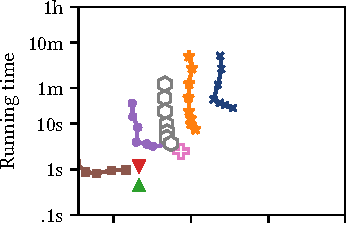
\includegraphics[scale=.7]{cost-running-time-tradeoff-1}%
    \hfill
    \vspace{-1ex}
    \caption{\queryref{1}\hspace{-2em}~}
    \label{fig:cost-running-time-tradeoff:1}
  \end{subfigure}
  \begin{subfigure}[t]{.2\linewidth}
    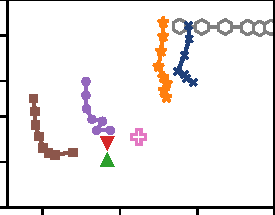
\includegraphics[scale=.7]{cost-running-time-tradeoff-2}%
    \hfill
    \vspace{-1ex}
    \caption{\queryref{2}\hspace{1em}~}
    \label{fig:cost-running-time-tradeoff:2}
  \end{subfigure}
  \begin{subfigure}[t]{.2\linewidth}
    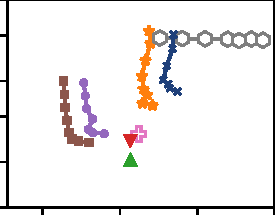
\includegraphics[scale=.7]{cost-running-time-tradeoff-3}%
    \hfill
    \vspace{-1ex}
    \caption{\queryref{3}\hspace{1em}~}
    \label{fig:cost-running-time-tradeoff:3}
  \end{subfigure}
  \begin{subfigure}[t]{.31\linewidth}
    \tikz[overlay,remember picture] \node[anchor=south west,inner sep=0]
      (cost-running-time-tradeoff-4) {
        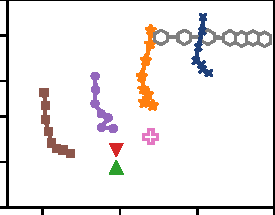
\includegraphics[scale=.7]{cost-running-time-tradeoff-4}};%
    \hfill
    \vspace{-1ex}
    \caption{\queryref{4}\hspace{7em}~}
    \label{fig:cost-running-time-tradeoff:4}
  \end{subfigure}
  \begin{subfigure}[t]{.245\linewidth}
    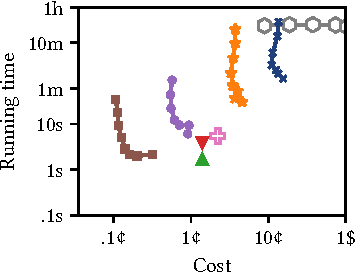
\includegraphics[scale=.7]{cost-running-time-tradeoff-5}%
    \hfill
    \caption{\queryref{5}\hspace{-2em}~}
    \label{fig:cost-running-time-tradeoff:5}
  \end{subfigure}
  \begin{subfigure}[t]{.2\linewidth}
    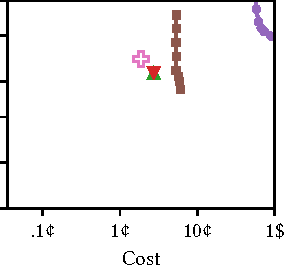
\includegraphics[scale=.7]{cost-running-time-tradeoff-6-1}%
    \hfill
    \caption{\queryref{6a}\hspace{1em}~}
    \label{fig:cost-running-time-tradeoff:6-1}
  \end{subfigure}
  \begin{subfigure}[t]{.2\linewidth}
    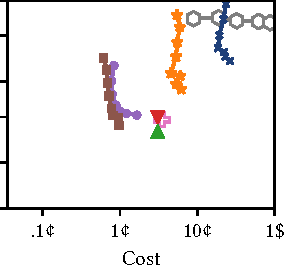
\includegraphics[scale=.7]{cost-running-time-tradeoff-7}%
    \hfill
    \caption{\queryref{7}\hspace{1em}~}
    \label{fig:cost-running-time-tradeoff:7}
  \end{subfigure}
  \begin{subfigure}[t]{.31\linewidth}
    \tikz[overlay,remember picture] \node[anchor=south west,inner sep=0]
      (cost-running-time-tradeoff-8) {
        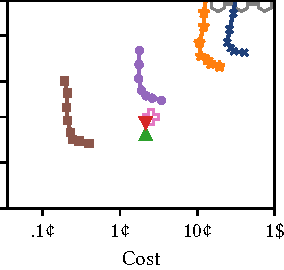
\includegraphics[scale=.7]{cost-running-time-tradeoff-8}};%
    \hfill
    \caption{\queryref{8}\hspace{7em}~}
    \label{fig:cost-running-time-tradeoff:8}
  \end{subfigure}%
  \caption{Running time/cost trade-off for various systems under test.}
  \label{fig:cost-running-time-tradeoff}
  \begin{tikzpicture}[overlay,remember picture]
    \node [fit=(cost-running-time-tradeoff-4)(cost-running-time-tradeoff-8),
           inner sep=0pt] (cost-running-time-tradeoff-right) {};
    \node [right=0em of cost-running-time-tradeoff-right,inner sep=0pt]
      (legend) {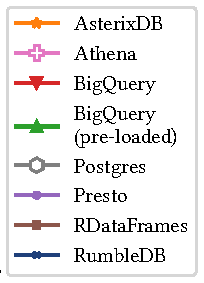
\includegraphics[scale=.7]{cost-running-time-tradeoff-legend}};
  \end{tikzpicture}
  \vspace{2ex}
\end{figure*}

\begin{figure*}
  ~\hspace{1em}
  \begin{subfigure}[t]{.25\linewidth}
    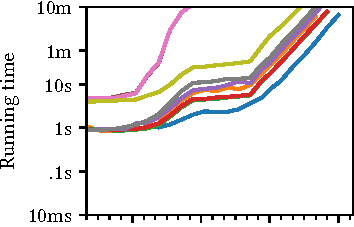
\includegraphics[scale=.7]{scaling-running-time-asterixdb}%
    \hfill
    \vspace{-1ex}
    \caption{AsterixDB\hspace{-3em}~}
    \label{fig:scaling-running-time:asterixdb}
  \end{subfigure}
  \begin{subfigure}[t]{.2\linewidth}
    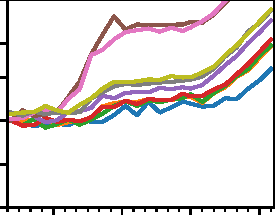
\includegraphics[scale=.7]{scaling-running-time-athena-v2}%
    \hfill
    \vspace{-1ex}
    \caption{Athena}
    \label{fig:scaling-running-time:athena-v2}
  \end{subfigure}
  \begin{subfigure}[t]{.2\linewidth}
    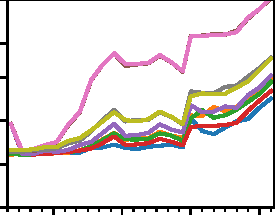
\includegraphics[scale=.7]{scaling-running-time-bigquery}%
    \hfill
    \vspace{-1ex}
    \caption{BigQuery (pre-loaded)}
    \label{fig:scaling-running-time:bigquery}
  \end{subfigure}
  \begin{subfigure}[t]{.27\linewidth}
    \tikz[overlay,remember picture] \node[anchor=south west,inner sep=0]
      (scaling-running-time-top-right) {
        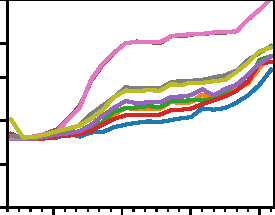
\includegraphics[scale=.7]
          {scaling-running-time-bigquery-external}};%
    \hfill
    \vspace{-1ex}
    \caption{BigQuery\hspace{5em}~}
    \label{fig:scaling-running-time:bigquery-external}
  \end{subfigure}
  \hfill~\\
  ~\hspace{1em}
  \begin{subfigure}[t]{.25\linewidth}
    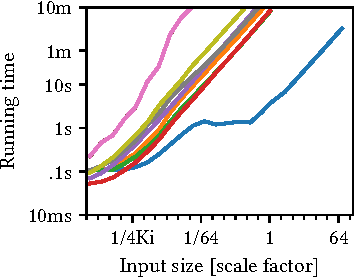
\includegraphics[scale=.7]{scaling-running-time-postgres}%
    \hfill
    \caption{Postgres\hspace{-3em}~}
    \label{fig:scaling-running-time:postgres}
  \end{subfigure}
  \begin{subfigure}[t]{.2\linewidth}
    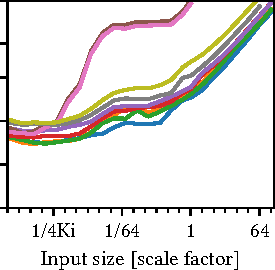
\includegraphics[scale=.7]{scaling-running-time-presto}%
    \hfill
    \caption{Presto}
    \label{fig:scaling-running-time:presto}
  \end{subfigure}
  \begin{subfigure}[t]{.2\linewidth}
    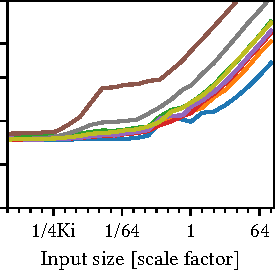
\includegraphics[scale=.7]{scaling-running-time-rdataframes}%
    \hfill
    \caption{RDataFrames}
    \label{fig:scaling-running-time:rdataframes}
  \end{subfigure}
  \begin{subfigure}[t]{.28\linewidth}
    \tikz[overlay,remember picture] \node[anchor=south west,inner sep=0]
      (scaling-running-time-bottom-right) {
        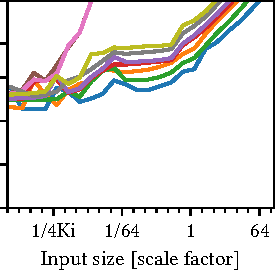
\includegraphics[scale=.7]{scaling-running-time-rumble}};%
    \hfill
    \caption{RumbleDB\hspace{6em}~}
    \label{fig:scaling-running-time:rumble}
  \end{subfigure}
  \hfill~
  \caption{Impact of data size on end-to-end running time
           of various systems under test.}
  \label{fig:scaling-running-time}
  \begin{tikzpicture}[overlay,remember picture]
    \node
      [fit=(scaling-running-time-top-right)(scaling-running-time-bottom-right),
       inner sep=0pt] (scaling-running-time-right) {};
    \node [right=0.5em of scaling-running-time-right,inner sep=0pt] (legend)
    {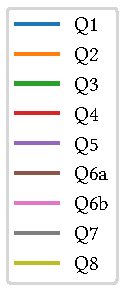
\includegraphics[scale=.7]{scaling-running-time-legend}};
  \end{tikzpicture}
\end{figure*}

\clearpage

\begin{figure}
  \centering
  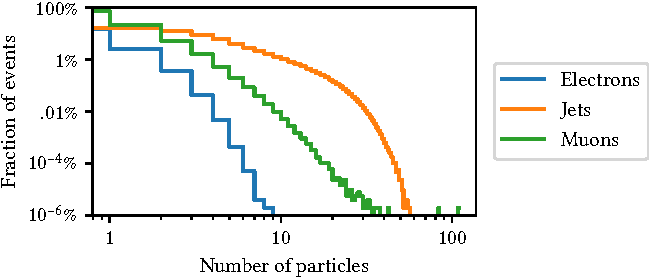
\includegraphics[scale=.7]{particle-distribution}
  \caption{Distribution of number of particles per event.}
  \label{fig:particle-distribution}
  \vspace{4ex}
\end{figure}

\begin{figure}
  \centering
  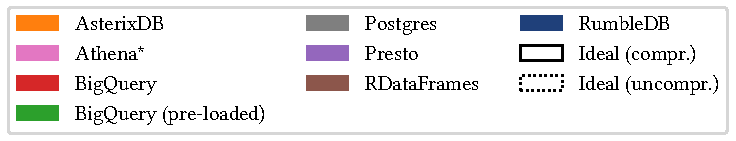
\includegraphics[scale=.7]{systems-legend}
  \begin{subfigure}[t]{\linewidth}
    \hfill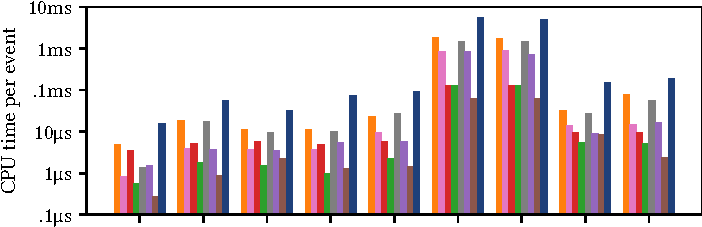
\includegraphics[scale=.7]{systems-cpu-time}
    \vspace{-1ex}
    \caption{Average CPU time per event.}
    \label{fig:systems:cpu-time}
    \vspace{1ex}
  \end{subfigure}
  \begin{subfigure}[t]{\linewidth}
    \hfill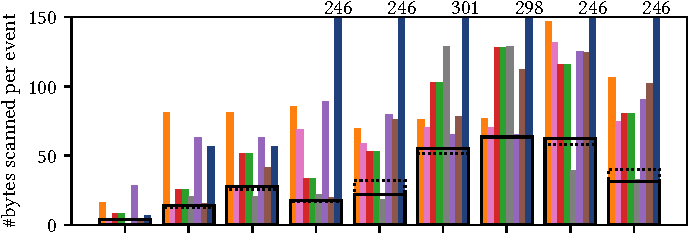
\includegraphics[scale=.7]{systems-data-scanned}
    \vspace{-1ex}
    \caption{Average amount of data scanned per event.}
    \label{fig:systems:data-scanned}
    \vspace{1ex}
  \end{subfigure}
  \begin{subfigure}[t]{\linewidth}
    \hfill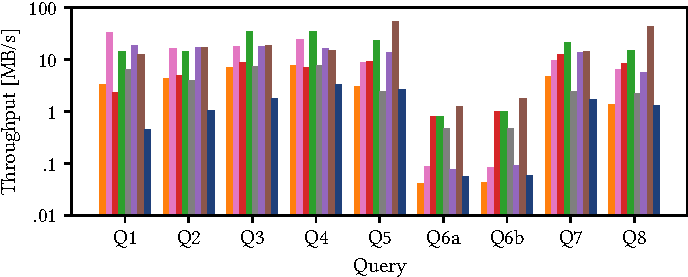
\includegraphics[scale=.7]{systems-scan-throughput}
    \vspace{-1ex}
    \caption{End-to-end processing throughput per logical core.}
    \label{fig:systems:scan-throughput}
  \end{subfigure}
  \caption{Analysis of compute/IO balance.}
  \label{fig:systems}
\end{figure}

\clearpage

\end{document}
